\documentclass[a4paper, 10pt]{article}
\usepackage[utf8x]{inputenc}
\usepackage[norsk]{babel}
\usepackage{natbib}
\usepackage{graphicx}
\usepackage[T1]{fontenc}
\usepackage{amsmath}
\usepackage{mathtools}
\usepackage{tabularx}
\usepackage{color, colortbl}
\usepackage{float}

\definecolor{Gray}{gray}{0.9}

\begin{document}
\begin{titlepage}
\begin{center} 

\vspace*{3cm}
\textsc{\Huge PU5}\\[0.7cm]
\textsc{\medium TTM4100 - Communication Services and Networks}\\[0.3cm]
\textsc{\medium TDT4140 - Software Enigneering}\\[0.3cm]
\textsc{\medium TDT4145 - Data Modeling, Databases and Database Management Systems}\\[0.3cm]
\textsc{\medium TDT4180 - Human-Computer Interaction}\\[0.3cm]

\textbf{\Large Gruppe 6:} \\[0.2cm]
\text{\Large Espen Albert, Finn Inderhaug, Kristoffer Andreas Dalby} \\
\text{\Large Christoffer B. Nysæter, Andreas Wien, Jonas André Dalseth}\\[1cm] 

\today

\end{center}
\end{titlepage}

\thispagestyle{empty}

\pagenumbering{roman}
\setcounter{page}{0}
\newpage
\tableofcontents

\newpage
\pagenumbering{arabic}
\setcounter{page}{1}

\section{Time}


\begin{tabularx}{\textwidth}{ |X|X|X| }
\hline
\rowcolor{Gray}
Task & Estimated hours & Registered hours \\ \hline
Create ER-diagram & 10 & 12 \\ \hline
Logic database schema & 10 & 10 \\ \hline
Setup the database server & 8 & 7 \\ \hline
Create SQL schema & 16 & 17 \\ \hline
Implement JDBC & 8 & 9 \\ \hline
Implement query methods & 16 & 20 \\ \hline
\hline
Planning server to client & 6 & 4 \\ \hline
Planning client to server & 6 & 4 \\ \hline
Server to clients, Master & 10 & 7 \\ \hline
Server and clients, Threads sending JSON objects to logged in clients & 16 & 12 \\ \hline
Clients to server, Master & 10 & 9\\ \hline
Clients to server, Check for inconsistency & 10 & 8\\ \hline
Clients to server, multiple Threads & 10 & 7\\ \hline
\hline
Creating login functionality & 7 & 7 \\ \hline
Parsing json objects to model & 8 & 9 \\ \hline
Define model and API structure  & 12 & 11\\ \hline
Create json objects based on the model & 8 & 9 \\ \hline
Creating vital functions and objects & 16 & 17 \\ \hline
Optimize the notify function & 15 & 12 \\ \hline    
\end{tabularx}


\begin{tabularx}{\textwidth}{ |X|X|X| }
\hline
\rowcolor{Gray}

Discuss how we want the user interface & 12  & 10\\ \hline
Designing the user interface using paper models & 12  & 14\\ \hline    
Show papermodel to studass and another group & 6  & 8\\ \hline
Fix papermodel after feedback & 3  & 5 \\ \hline
Conceptual model & 6  & 4\\ \hline
Screen design & 12  & 12\\ \hline
Construction design & 12  & 12\\ \hline
Make login screen & 4  & 5\\ \hline
Make appointment view & 16  & 14\\ \hline
Make week view & 16  & 18\\ \hline
Other functionality & 16  & 16\\ \hline
\hline
Administration & 0 & 10 \\ \hline
PU1 & 0 & 41 \\ \hline
PU2 & 0 & 41 \\ \hline
User interface discuss & 0 & 4 \\ \hline
Paper model & 0 & 26 \\ \hline
Show papermodel & 0 & 10 \\ \hline
PU1-3 eval & 0 & 5 \\ \hline
Java helperclasses & 0 & 2 \\ \hline
MMI Report & 0 & 14 \\ \hline
Java FX screen design & 0 & 81 \\ \hline
PU5 & 0 & 11 \\ \hline
D3 & 0 & 24 \\ \hline
Testing and debugging & 0 & 7 \\ \hline


\end{tabularx}

\subsection{Unexpected tasks}
As you can see in the table, the last rows are task we did not think of as of the planning in the PU1 assignment. Some of those task took us by surprise and took very long to finish. This had a major impact on the projects work breakdown schedule. 

\subsection{Java FX}
We tried to use Java FX because it was the newer, more modern UI framework. This was not that easy as we though and unexpected problems ended up taking up a lot of time, which affected the product and made testing hard.

\subsection{Loss of manpower}
Throughout the project we had a problem with one of the group members being sick, over most of the project period. This resulted in loosing 14 days worth of work. We have also had team members that had other meetings to go to which also eat away from our work hours. The occasional sickness also targeted us by taking out a member for 4 days. To make up for the lost work power the members that was able to meet worked longer days at the end. We worked approximately 32 hours a day, and at the end we worked up to 43 hours a day. Our plan was originally to work around 36 hours a day.

\begin{figure}[h!] 
    \begin{center} 
    	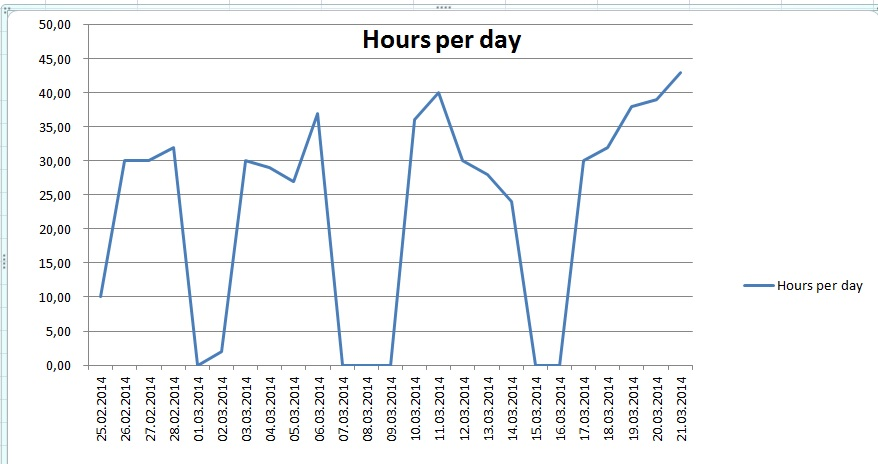
\includegraphics[width=15cm]{hoursPerDay.jpg}
		\caption{Work hours per day}
	\label{gantt}
	\end{center}
\end{figure}

\section{Systemtesting}
\subsection{Results}
\begin{tabularx}{\textwidth}{ |X|X|X| }
\hline
\rowcolor{Gray}
Test & Number & Success \\ \hline
Log in & \# 1 & Yes \\ \hline
Add appointment & \# 2 & Yes \\ \hline
Respond & \# 3 & - \\ \hline
Edit appointment & \# 4 & Yes \\ \hline
Delete appointment & \# 5 & - \\ \hline
Book room & \# 6 & - \\ \hline
View & \# 7 & Yes \\ \hline
Check status & \# 8 & -  \\ \hline
Decline invitation & \# 9 & - \\ \hline
Book room & \# 10 & - \\ \hline
View & \# 11 & Yes \\ \hline
Track invite & \# 12 & - \\ \hline
View other calendars & \# 13 & Yes \\ \hline
Alarm & \# 14  & - \\ \hline

\hline


\end{tabularx}

\subsection{Out of time}
We did not have time to finish all the functionality of the program, most of the requirements are nearly done, but we did not have time to finish the implementation of all of them. And therefor there was not any time to test it.

\subsection{Changes}

\section{Experiences}

\subsection{Negative experiences}
\subsubsection{Bad communication}
A negative experience from this project has been bad communication between the members in the group, especially with the members that has been sick or unavailable a lot. This has resulted in many a lot of working hours that has just been used for catching up and updating them unnecessary. Between the group members that have been meeting regularly the problem has been mainly that they have not spoken of what they are doing and how far they have come. This has resulted in a little unbalance workload between some parts of the program. Another problem has also been that people has not asked for help instead of hitting the wall with a problem over and over.
\subsubsection{Meeting in time}
A problem for most members in the group is to meet at time, or meeting at all. Very many members are deep sleepers, and sleep right through their alarm. This has resulted in many meetings not starting as late as one hour after the agreed meeting time.

\subsection{Positive experiences}
\subsubsection{New friends}
The members of the group has come very well along right from the start. And we would all say that a very positive experience is that we have been able to make friends across the different studies we are enrolled in. A very good thing about this is that we have been able to work together closely every day in a longer time periode without wanting to kill one another.

\subsubsection{New knowledge}
From the first meeting we had we discussed the different roles that coding the project would include and who was interested in what. Every member quickly selected a main area they wanted to focus on and everyone got to work with what they wanted. By choosing an assignment that a member would like to work on, the productivity was rather good. At the point of writing this, every member is really satisfied with all the new knowledge they have gained. The practice experience in the area of databases, graphical interfaces and networking is very good for the future.



\subsection{What could we do better?}
\subsubsection{Scrum meetings}
Our group have not been very good with regular scrum meetings, this is definitely something we could do better. We see that the negative experiences from bad communication would probably have been eliminated if regular scrum meetings was something we did every day. We ended up with trying to catch up with everything when we had meeting, which resulted in long inefficient meetings. 
\subsubsection{Group leader}
Every group did get a group leader which was assigned by the teaching staff. The group in general did not use this person as the leader, instead we all took responsibility, which in the start worked very well. But at the end of the project it was hard for everyone to keep up with all the loose ends and what need to be done in what order.  Since we had no one that had the overview over the big picture it was really hard to assign the different issues that still was around to the people that did not have anything to do. When we look at this problem in retrospective it is easy to see that the group leader role should be assigned and given specific task to do as we went through the project.

\subsubsection{Deadlines}
Another thing we should have done is to create and work with deadlines throughout the project. We did not have any deadlines except the due dates for every assignment, which actually was a problem when we started to code and did not have regular due dates.

\end{document}
